\documentclass[11 pt]{article}
\usepackage{amsmath,amsfonts,parskip}
\usepackage[a4paper]{geometry}
\usepackage[T1]{fontenc}
\usepackage{enumerate}
\usepackage{graphicx}
\usepackage{cleveref}

\begin{document}

\begin{center}
       \large{
       \textbf{Computational Physics - PH3264} \break
	Module 2 - Integration
}
\end{center}

\textbf{Krishna Iyer V S \hfill Roll:20201017}
\hrule 
\vspace{0.3cm}
\begin{enumerate}
\item
\begin{enumerate}[a.]

\item  The error is measured as $\text{abs}(\pi - \text{estimate})$, indicating that we our approximation does indeed approach $\pi$.

\item The function's actual integrand is $\pi$. The following plot shows the errors plotted against the number of bins on a log-log scale.
\begin{figure}[h]
\begin{center}
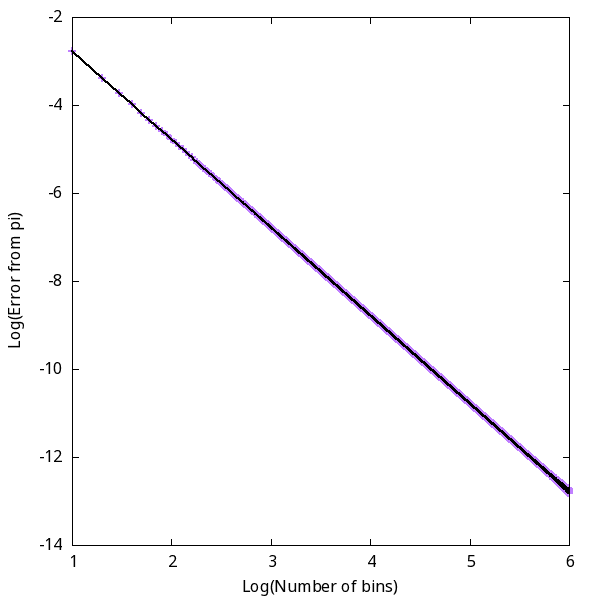
\includegraphics[width=2.5in]{"plots/log_log_q1_a.png"}
\end{center}
\end{figure}
		The slope of the line is -1.9998, which is close to what is predicted by theory (predicted slope: -2).

\item Taking $sin(x)$ with 10,000 bins, the value estimated is 2 - which agrees with the theory and confirms that the integration scheme works. 

\item The answer obtained is 0.997300 which appears to match with gaussian integral tables.
\end{enumerate}

\item
\begin{enumerate}
\item
The random numbers plotted as a histogram with bin size is shown in Figure \ref{fig2} (left) - suggesting that the random numbers are uniform.
\item
The first 10000 (out of 100,000) random numbers are plotted on a scatter plot in Figure \ref{fig2} (right).
\begin{figure}[h]
\begin{center}
\label{fig2}
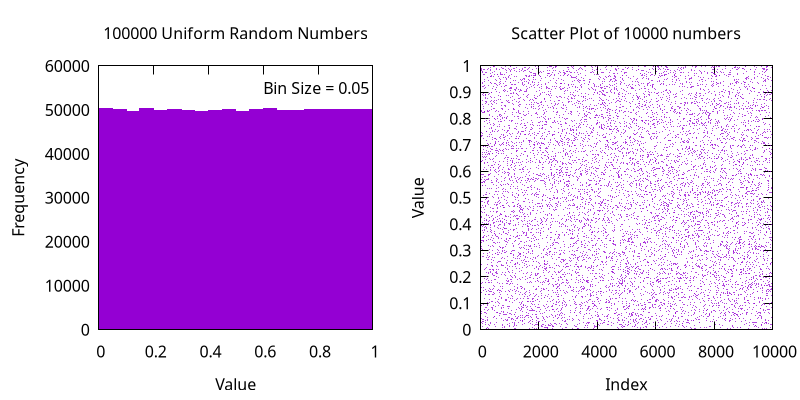
\includegraphics[width=3.8in]{"plots/q2_ab.png"}
\end{center}
\end{figure}
\item
The auto-correlation function plotted with increasing lag is shown in Figure \ref{fig3}. The auto-correlation function has the following form:
\[
\hat{R(k)}=\frac{1}{(n-k)\sigma^2}\sum_{t=1}^{n-k} (X_t-\mu)(X_{t+k}-\mu)
\] 
\begin{figure}[h]
\begin{center}
\label{fig3}
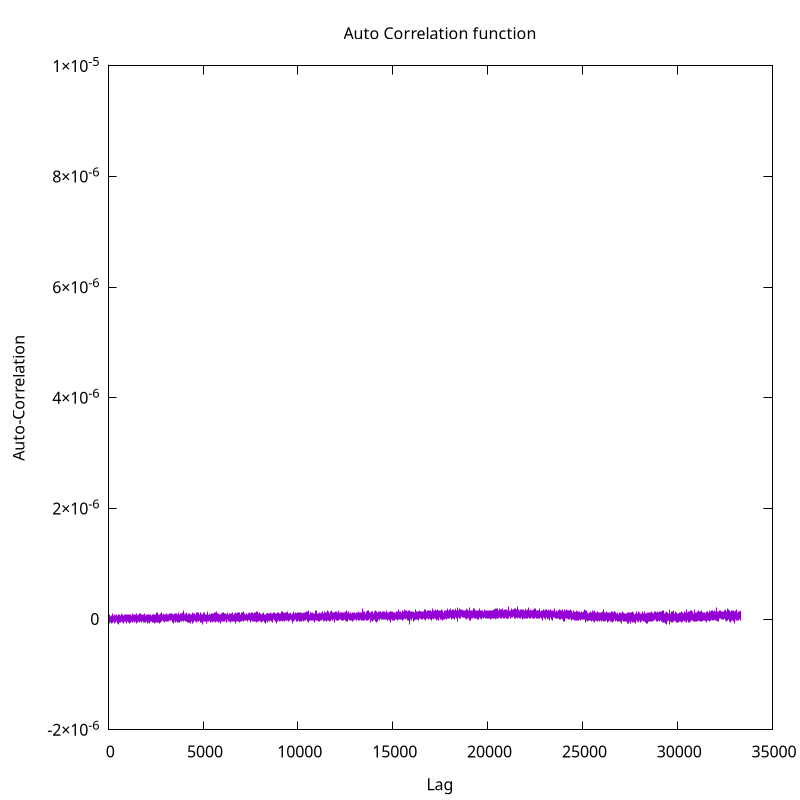
\includegraphics[width=2.5in]{"plots/q2_c_correlation.png"}
\end{center}
\end{figure}

\item The mean and standard deviation of this uniform distribution are 0.5001 and 0.28879.
\end{enumerate}
\item
\begin{enumerate}
\item For generating a random variable that samples according to the distribution $e^{-2x}$, we scale uniformly generated random numbers by $-2\cdot ln(1-x)$. The distribution generated by this random device is shown in Figure \ref{fig4}.
\begin{figure}[h]
\begin{center}
\label{fig4}
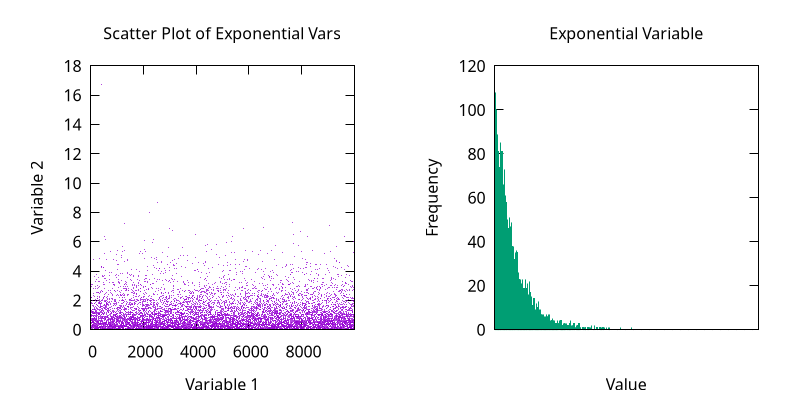
\includegraphics[width=5in]{"plots/q3_a_exponential.png"}
\end{center}
\end{figure}
\item For generating random numbers with a gaussian distribution, we use the Box-Muller transform to convert a set of numbers in a 1x1 square to a set of exponentially distrubted numbers in the XY plane, such that any orthagonal axis is an independent variable.
\begin{figure}[h]
\begin{center}
\label{fig4}
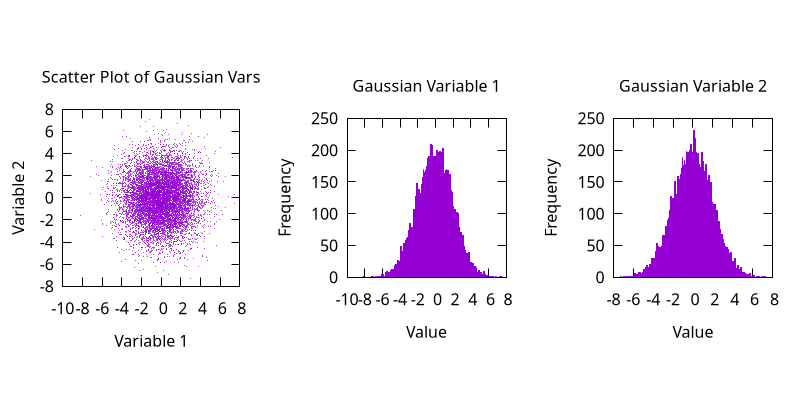
\includegraphics[width=5in]{"plots/q3_b_gaussians.png"}
\end{center}
\end{figure}
\end{enumerate}
\item
\begin{enumerate}
\item Brute Force Integration.
\begin{verbatim}
10      03.4258   4.706778
100     11.9365   6.961318
1000    10.8966   2.375228
10000   10.8879   0.742370
100000  10.8913   0.234514
\end{verbatim}
\item Importance Sampling.
\begin{verbatim}
10      11.8298   3.316574
100     11.0888   0.927880
1000    10.9777   0.230598
10000   10.9629   0.079027
\end{verbatim}
\end{enumerate}
\end{enumerate}
\end{document}
